\section{Conception d'une plateforme pour les chercheurs}
    \subsection{Utilisation des sources du droit chinois en humanités numériques}

L'accès aux sources du droit chinois, au croisement entre les disciplines que sont l'histoire et le droit, est encore peu développé. Les collections de la bibliothèque d'études chinoises du \cdf contient les textes de lois du corpus du projet mais la bibliothèque étant en travaux, la consultation sur place n'est possible que sur rendez-vous. Sur le web, certains projets proposent un accès aux sources mais celles-ci restent majoritairement partielles. Le projet \LSC  propose une édition trilingue des codes légaux chinois de la dynastie Qing, cependant les données ne sont pas complètes à l'heure actuelle et les documents sont toujours en cours de saisie sur le site internet. Le projet de recherche japonais \textit{Terada's Homepage for Chinese Legal History Studies in Japan} \footnote{http://www.terada.law.kyoto-u.ac.jp/index_en.htm} de l'Université de Kyoto propose une édition du \dc uniquement. Or, l'étude du droit chinois et de son évolution nécessite la consultation simultanée des différents textes de lois. La conception d'un site web réunissant ces sources dans leur intégralité afin de faciliter l'accès aux chercheurs est donc au centre du projet \COREL. 

De plus, ces projets de recherche offrent uniquement un accès à leur édition en ligne, mais l'histoire du droit chinois est une discipline peu développée en humanités numériques. Les données et leur éditorialisation ne sont que peu diffusées en \textit{open access}. La production de données \textit{open source} par le projet \COREL cherche à permettre aux humanités numériques de s'approprier ce terrain de recherche et de favoriser le développement de projets de recherche sur la généalogie du droit. Cependant, des outils \textit{open source} se développent peu à peu dans les projets d'humanités numériques. La version bêta de \textit{MARKUS}, en cours de développement par l'Université de Leyde aux Pays-Bas, permet le balisage et le référencement des entités nommées pour les textes chinois. Dans le cadre du projet \COREL, nous avons également testé le script \textit{Chinese Calendar Tools} \footnote{https://gitlab.com/vandenbosch.nora/chinesecalendartools/-/tree/main}, qui permet de convertir les dates du calendrier luni-solaire chinois \footnote{Le calendrier luni-solaire, utilisé par plusieurs cultures, est un calendrier combinant le calendrier lunaire et solaire.} vers des dates du calendrier grégorien. Bien que l'échéance du financement n'ait pas permis d'exploiter ces deux outils \textit{open source} afin d'enrichir l'encodage des sources, ils permettent de démontrer que les études chinoises dans les humanités numériques en Europe se développent peu à peu. Le projet \COREL s'inscrit dans cette démarche de science ouverte et contribue avec l'éditorialisation du corpus de codes légaux de la dynastie Qing et la mise à disposition en \textit{open access} de ces données, au développement des projets d'humanités numériques pour les études chinoises. 

\subsection{Les enjeux de la reconstitution de la législation}

Offrir une édition scientifique numérique complète des textes légaux sous la dynastie Qing est donc un projet conséquent qui ambitionne de faciliter l'accès aux sources par les chercheurs, en concevant une plateforme unique réunissant les sources pour une consultation simultanée des textes. L'édition numérique permet à la fois de réunir les différents volumes d'un même code légal, mais aussi de proposer sur le même site web toutes les sources de droit chinois sous la dynastie Qing dont dispose le projet.

Toutefois, l'éditorialisation du corpus n'est qu'une partie du projet \COREL. En effet, l'équipe souhaite reconstituer la législation de 1644 à 1911, pour chaque année de la dynastie Qing. La recréation d'un texte de loi, généré automatiquement à la demande des utilisateurs, permettrait de faciliter l'accès aux sources à un niveau supérieur. À l'instar des nombreuses compilations rédigées sous la dynastie Qing, le \cv permettrait de compiler en temps réel toutes les lois valides pour une année donnée. Cet aspect du projet vise à faciliter les recherches de l'évolution du droit par le numérique : plutôt qu'un travail de recherche comparatif entre les différents textes, les chercheurs auront accès à la reconstitution de la législation grâce à l'agrégation de toutes ces sources, directement sur le web, en libre accès. 

Enfin, la reconstitution de la législation s'accompagne d'un travail sur la généalogie des lois. Les visualisations via les liens d'association dirigée entre les lois permettront également de faciliter le travail de recherche en retraçant la généalogie d'une loi en entier, sans nécessité de naviguer entre les différentes sources partielles. En effet, pour étudier la généalogie des lois, une étude de toutes les sources est nécessaire afin de trouver toutes les versions de la loi et ses modifications dans le temps, jusqu'à son abrogation. Aucun accès immédiat à la généalogie complète d'une loi n'est disponible dans les textes, puisque toutes les sources sont partielles et se complètent les unes les autres. Le projet \COREL ambitionne donc d'aider les chercheurs en facilitant ce travail de recherche sur la généalogie des lois. 

\subsection{Définition des besoins utilisateurs}

Le public cible du projet étant les chercheurs en histoire du droit chinois, il est possible d'établir des besoins utilisateurs précis pour le projet \COREL. D'une part, les chercheurs doivent pouvoir accéder à l'édition scientifique numérique des sources sur le site web, avec une structure des textes qui leur est familière, c'est-à-dire que l'édition des textes de lois doit se faire, à l'instar de la source originale, en chapitres et sections. Chaque chapitre, sections et les différentes lois doivent être numérotés afin de se repérer dans les textes. Les chercheurs ont aussi besoin de pouvoir naviguer entre les différents textes, le corpus se prêtant à de la consultation plutôt qu'à une lecture continue et linéaire. Une table des matières cliquable et qui indique la position actuelle de l'utilisateur doit donc être créée. 

En plus de l'édition en ligne, les utilisateurs doivent pouvoir accéder à la recréation de la législation, le \cv, afin de pouvoir accéder à un texte de loi composite pour une année entre 1644 et 1911. Un format \pdf doit être disponible au téléchargement pour être consulté hors connexion. Cette reconstitution de la législation doit respecter la mise en page d'un texte de lois, c'est-à-dire qu'il doit présenter les chapitres et sections usuels. Le besoin des chercheurs n'est pas de filtrer simplement les données par dates, mais de conserver la structure des codes afin de pouvoir consulter, par exemple, les lois selon les ministères auxquels elles sont rattachées, ou encore les \li selon la loi principale qu'elles viennent compléter. 

Enfin, une modélisation des liens d'association dirigée entre les lois est essentielle afin de faciliter les travaux de recherche et d'offrir une compréhension instantanée de la généalogie d'une loi. En effet, le fichier de référencement des liens entre les lois tels qu'il existe actuellement pour appuyer le projet demeure difficile d'appréhension à la première lecture et demande de naviguer via les liens hypertexte. La lecture de ce document, qui n'est pas continue, ne permet pas de saisir immédiatement la généalogie d'une loi. Apporter des visualisations aux utilisateurs est donc un besoin primordial afin de faciliter les recherches sur la généalogie des lois et leur évolution. 

Afin de répondre aux besoins des chercheurs, qu'ils soient utilisateurs ou administrateurs, il est important de concervoir une plateforme adaptée, en libre accès, afin de contribuer au développement de l'histoire du droit chinois en humanités numériques.

 \section{La publication de données en ligne : un travail accessible à un plus large public}
    \subsection{L’outil TEI Publisher}
\tp est un outil de publications de données encodées en \TEI, qui s'appuie sur le système de gestion de base de données \XML \textit{eXist-db}. C'est un outil \textit{open source} qui propose de construire une édition en ligne, essentiellement en interface graphique. Des templates \HTML sont ensuite générés, ce qui permet aux chercheurs de publier leurs corpus de recherche édités en codant le moins possible. Il est également possible de publier d'autres langages via  \tp : le \XML Docbook, \JATS ou encore les fichiers .docx. L'outil \tp respecte des standards afin de faciliter l'échange des données et les principes \fair en utilisant les langages \XML (\TEI, \ODD, XQuery). La construction d'un site web à partir de l'application \tp est possible grâce à la génération des templates \HTML et de l'utilisation des \textit{webcomponents}, qui font partie des spécifications \HTML 5 afin de personnaliser le site web. Afin d'offrir un haut niveau de personnalisation tout en garantissant la pérennité des sites web construits à partir de \tp, l'application propose d'utiliser les \textit{webcomponents} comme des briques individuelles à ajouter et assembler selon les besoins utilisateurs. 

L'usage de \tp se démocratise de plus en plus dans les projets en humanités numériques. Le site web du projet \cordel (mais aussi les projets menés par l'INRIA), a été construit via \tp. L'utilisation de \tp a donc été envisagée dès le début du stage, afin d'organiser une veille sur cet outil. Cette veille s'est organisée en trois temps : 

\begin{itemize}
    \item La consultation de la documentation de \tp et des applications réalisées, notamment \cordel et \disco. 
    \item La réalisation de deux entretiens avec Hugo Scheithauer (en visioconférence) et Floriane Chiffoleau (à l'INRIA). 
    \item Un test via l'\og aire de jeux \fg de \tp, qui permet de tester immédiatement les fonctionnalités de l'application en local. 
\end{itemize}

\subsubsection{La documentation}
\tp dispose d'une documentation complète \footnote{https://teipublisher.com/exist/apps/tei-publisher/doc/documentation.xml?odd=docbook\&view=div} consultable en ligne. En plus de la documentation écrite, il existe des cours en ligne, \og Stay home and learn \TEI from scratch \fg, proposé par \textit{e-editiones}, un groupe à but non lucratif qui oeuvre pour le développement de la science ouverte dans l'édition scientifique numérique. La documentation étant longue et exhaustive, cette première étape de la veille sur \tp s'est étalée sur plusieurs semaines en début de stage afin de se familiariser avec la méthodologie générale de la création d'un site web via \tp. La consultation ponctuelle de la documentation et des cours en ligne s'est par la suite révélée indispensable tout au long du stage, afin de compléter cette première approche, notamment lors de la mise en pratique. 

\subsubsection{Entretiens avec des professionnels}
En plus de la consultation de la documentation, j'ai mené deux entretiens à propos de \tp. Le premier, avec Hugo Scheithauer, à propos de l'application Data Catalogue, un projet d'édition scientifique numérique de catalogues de vente, m'a permis d'obtenir des informations générales sur la méthode de travail et la gestion d'un projet avec \tp : un tel projet est généralement mené en équipe de deux, avec un développeur \textit{front-end} et un développeur \textit{back-end}. L'utilisation de \tp, bien qu'en interface graphique, requiert des connaissances minimales en développement web et en langages \XML. M. Scheithauer a également souligné l'importance de la préparation des données avant le démarrage du projet. \textit{A priori}, avec toutes les données nécessaires identifiées et ajoutées dans l'encodage et une équipe de deux personnes, il est possible de créer un site web simple assez rapidement\footnote{Bien qu'il soit difficile d'estimer les délais de conception, qui sont propres à chaque projet, M. Scheithauer a indiqué qu'il envisageait un délai d'environ six mois pour se consacrer au développement d'une application simple, à partir d'une équipe de deux personnes}. Toutefois, si l'on souhaite un haut niveau de personnalisation pour le site web, il est probable qu'il soit nécessaire d'intervenir sur le code source de l'application directement.

Un second entretien avec Floriane Chiffoleau, à propos du projet \disco, m'a permis d'approfondir ma compréhension du fonctionnement de \tp et de découvrir les méthodes de travail derrière \disco. Mme Chiffoleau m'a parlé de sa propre expérience avec \tp : elle a consacré deux semaines à la consultation de la documentation de \tp, en ayant déjà une bonne maîtrise des langages \XML, puis un mois de tests de l'application. Elle m'a présenté les différents modes d'affichage des éditions \disco, chacun permettant de mettre en lumière des informations différentes. Trois modes sont présents sur l'application \disco : un mode pour l'édition critique, un pour l'édition diplomatique et enfin un mode permettant de mettre en valeur les entités nommées. Ce dernier mode est également envisagé à ce jour pour la réalisation du projet \COREL. 

\begin{figure}[h]
    \centering
    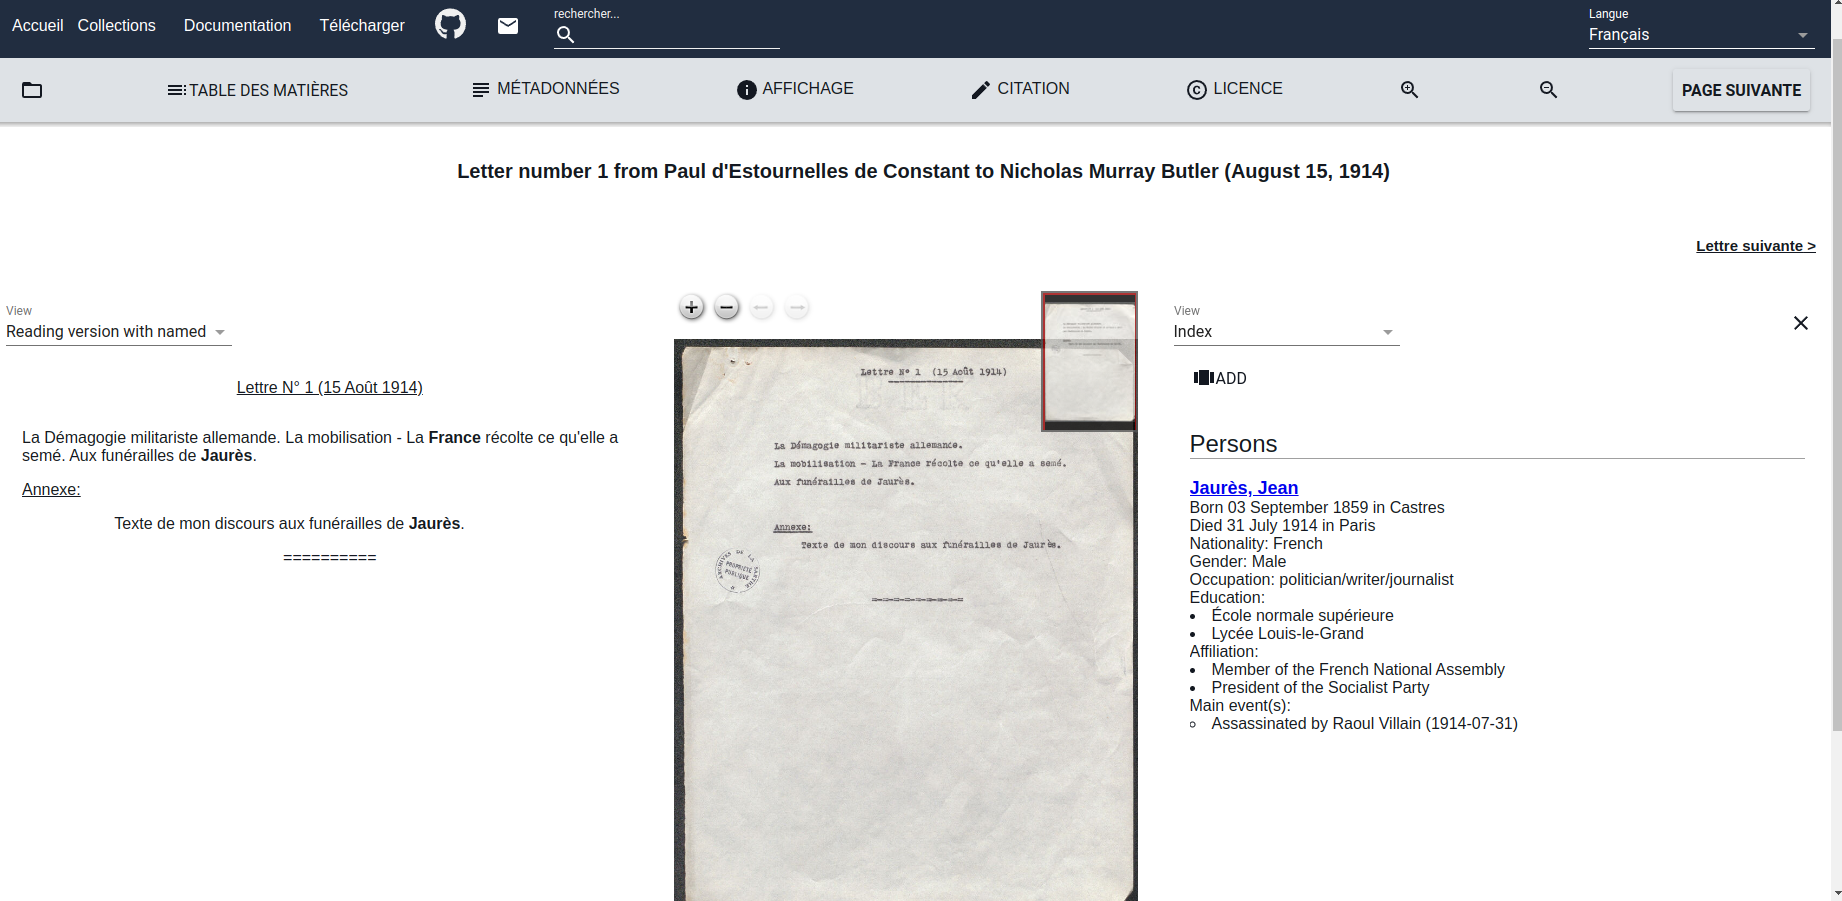
\includegraphics[width=\textwidth]{images/discholed.png}
    \caption{Capture d'écran du site web \disco}
\end{figure}

Lors de cet entretien, elle a également pu souligner l'importance d'encoder des documents \TEI valides, avec des règles de validations précises dans l'\ODD. En effet, si les documents ne respectent pas les mêmes règles de validation, cela complexifie le processus de conception de l'application, étant donné que \tp permet d'attribuer un comportement à un élément (par exemple, les balises \texttt{<note>} du corpus \COREL s'affichent en bleu). Ainsi, respecter un schéma d'encodage défini permet de prévenir des erreurs d'affichages. 

Une fois ces deux premières étapes de veille menées à bien, l'aire de jeux \tp a permis d'effectuer un premier test avec le jeu de données \TEI de référence. 

\subsection{L’édition scientifique en interface graphique}

\tp permet en effet de construire son site web en interface graphique, grâce à une \ODD. L'\ODD \tp n'est pas à confondre avec l'\ODD qui permet de documenter un projet d'encodage et de définir des règles de validation. L'\ODD \tp est à distinguer d'une \ODD classique, puisqu'elle permet d'attribuer à un élément un comportement (\og behaviour \fg), c'est-à-dire une manière de s'afficher. Grâce à des requêtes XQuery générées automatiquement par \tp, les balises \TEI sont attribuées l'affichage souhaité sur le template \HTML. Il est possible de tester directement cette fonctionnalité grâce à l'aire de jeux de l'application \tp, une interface qui permet d'accéder à différentes \ODD d'exemples, comme pour les correspondances de Van Gogh ou les pièces de Shakespeare.\footnote{Les correspondances de Van Gogh et les pièces de Shakespeare sont deux éditions numériques publiées qui sont utilisées comme exemples par \tp.} L'aire de jeux donne l'accès aux \ODD et permettent de les modifier afin de tester les différentes possibilités d'affichage offertes par \tp. Il est possible de télécharger ses propres documents sur l'aire de jeux et de tester les \ODD disponibles, en les modifiant pour les adapter aux documents. Il est également possible de créer sa propre \ODD.

\begin{figure}[h]
    \centering
    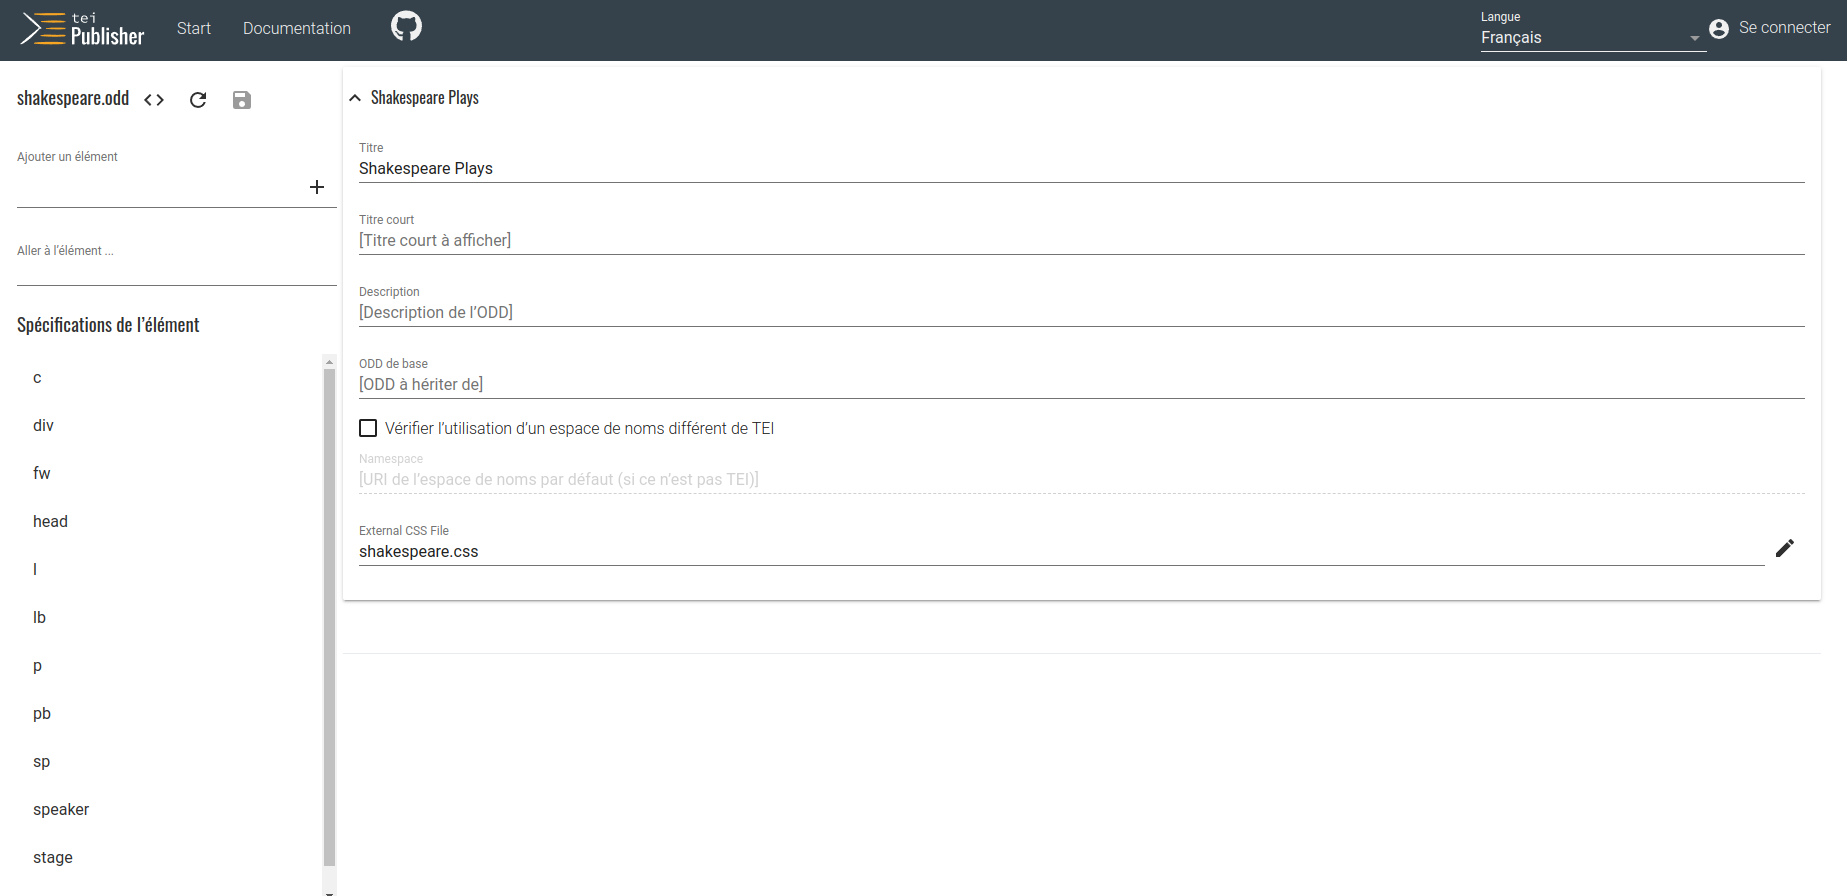
\includegraphics[width=\textwidth]{images/playground.png}
    \caption{Capture d'écran de l'aire de jeux \tp}
\end{figure}

La modification de l'\ODD est accessible intégralement en interface graphique. Ce mode d'édition est conseillé pour les débutants. Sur la gauche, il est possible de sélectionner les balises dont on veut modifier le comportement. Grâce à un chemin \xpath et à du code \CSS, \tp lance ensuite une requête XQuery qui applique le comportement choisi dans les templates \HTML générés automatiquement. 

\begin{figure}
    \centering
    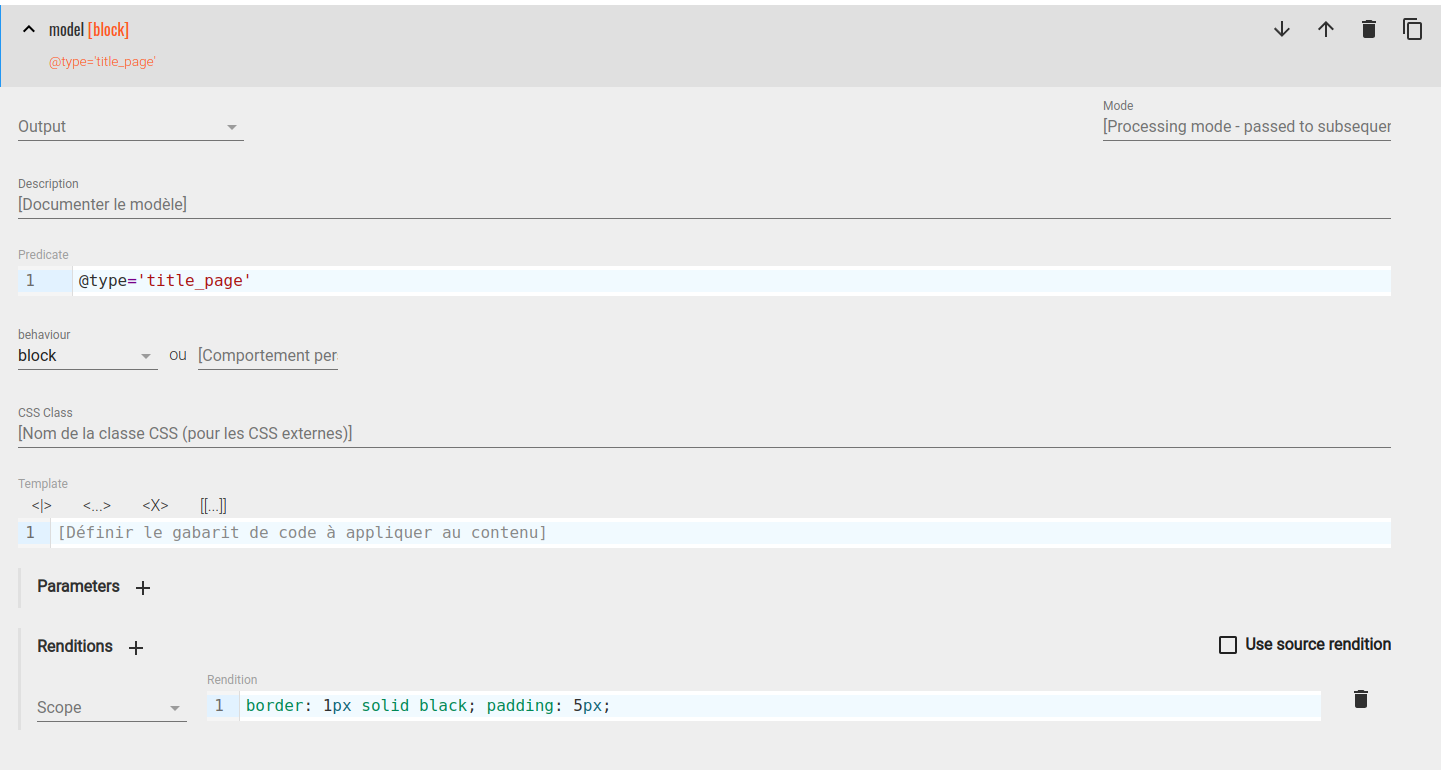
\includegraphics[width=\textwidth]{images/odd_playground.png}
    \caption{Capture d'écran de l'aire de jeux \tp : modifier le comportement d'un élément}
\end{figure}

Il est également possible d'éditer l'\ODD directement dans le code \XML. Ce mode d'édition nécessite cependant une connaissance avancée des langages \XML et une bonne compréhension du \textit{\TEI Processing Model}, qui est le langage derrière l'\ODD de \tp. Le \TEI Processing Model fait partie des \textit{guidelines} \TEI et leur documentation est donc accessible en ligne. 

L'objectif du projet \COREL étant de produire une édition scientifique numérique le plus possible en interface graphique, c'est le premier mode d'édition de l'\ODD qui a été jugé le plus pertinent pour le projet. Dans le cadre du stage, un premier test de cette fonctionnalité de \tp a donc été réalisé, afin de reproduire l'un des différents modes d'affichages souhaités pour le projet.\footnote{À propos de ces différents modes d'affichages, voire la partie concernée dans le cahier des charges, en annexes.} 

\begin{figure}[h]
    \centering
    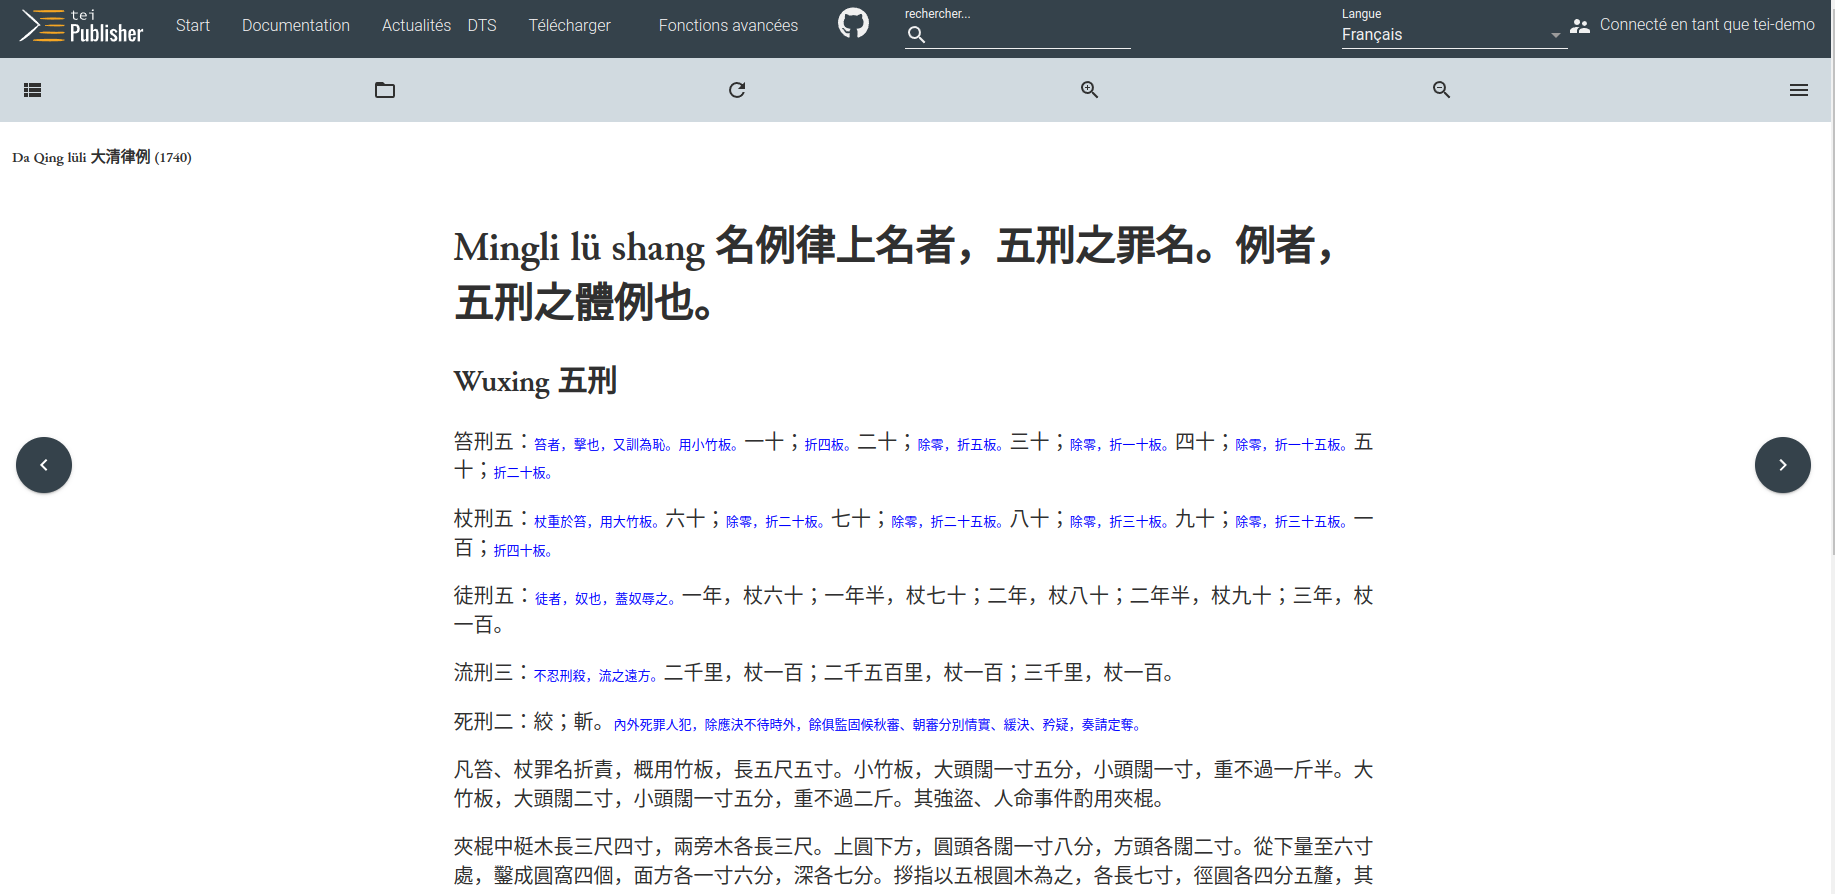
\includegraphics[width=\textwidth]{images/tei_publisher_test.png}
    \caption{Capture d'écran du résultat du test de l'aire de jeux}
\end{figure}

Le mode d'affichage principal souhaité par le projet permet de mettre en avant les commentaires officiels contenus par les textes de lois, en caractères bleus de police inférieure au texte principal. Ces commentaires, contenus dans des balises \texttt{<note>} ont été sélectionnés via un chemin \xpath : \texttt{@type='official'}. En effet, les textes contiennet plusieurs types de commentaires. Seuls les commentaires officiels ont été sélectionnés afin de leur attribuer un comportement. Par défaut, \tp traite les balises \texttt{<note>} comme des notes de bas de page, via le comportement \textit{note}. Afin de les affichers au sein du texte, il a fallu modifier le comportement par défaut et sélectionner le comportement \textit{inline}, qui permet d'afficher les balises au sein du texte. Ensuite, le code \CSS suivant a permis d'afficher ces commentaires en bleu dans une police inférieure : 

\begin{minted}{css}
    font-size: small; color: blue;
\end{minted}

L'aire de jeux \tp est donc un moyen efficace de tester les fonctionnalités offertes par l'application avant de démarrer un projet. Grâce à la veille informationnelle puis au test effectué lors du stage, il a été possible de déterminer que \tp semble être un outil compatible avec les besoins du projet et la réalisation des livrables. Cependant, il est également possible de souligner les limites de \tp. En effet, bien qu'entièrement réalisable en interface graphique, l'édition scientifique numérique via \tp nécessite une bonne maîtrise des langages \XML et du développement web, notamment \HTML et \CSS. La réalisation d'un site web via \tp permet de passer moins de temps à coder et de créer une édition dans le respect des normes d'interopérabilité et de pérennité des données sur le web. Cependant, la prise en main de l'outil n'est pas instantanée et nécessite des compétences techniques minimales et un temps de formation. Si les chercheurs auront la possibilité d'ajouter et de modifier des documents sans problème en \XML, via l'interface eXist, il leur sera plus difficile de paramétrer les modes d'affichages seuls, malgré l'interface graphique de \tp. 

